\documentclass[11pt,a5paper]{article}

\usepackage[T1]{fontenc}
\usepackage[utf8]{inputenc}
\usepackage{lmodern, microtype}
\usepackage[estonian]{babel}
\usepackage[per=fraction, expproduct=cdot, decimalsymbol=comma, inter-unit-product=\cdot]{siunitx}
\usepackage{graphicx}
\usepackage{wrapfig}
\usepackage{subfig}
\usepackage{tikz}
\usetikzlibrary{arrows.meta}
\usepackage[european]{circuitikz}
\tikzset{component/.style={draw,thick,circle,fill=white,minimum size=0.75cm,inner sep=0pt}}
\usepackage{amsmath,amssymb}
\usepackage{amsfonts}
\usepackage[hidelinks]{hyperref}
\usepackage{csquotes}
\usepackage{caption}
\usepackage{enumitem}
\topmargin=-3.0cm \textheight=19cm \textwidth=12.9cm
\oddsidemargin=-1.5cm  \evensidemargin=-1.5cm
\setlength{\parindent}{0pt} \setlength{\parskip}{6pt} \sloppy
\sloppy \relpenalty=10000 \binoppenalty=10000
\pagestyle{empty}

\newcommand{\numb}[1]{\vspace{5pt}\textbf{\large #1}}
\newcommand{\nimi}[1]{(\textsl{\small #1})}
\newcommand{\punktid}[1]{(\emph{#1~p.})}
\newcounter{ylesanne}
\newcommand{\yl}[1]{\addtocounter{ylesanne}{1}\numb{\theylesanne.} \nimi{#1} \newblock{}}
\newcommand{\autor}[1]{}% Kasuta võistluse ajal
%\newcommand{\autor}[1]{\emph{ Autor: #1}}% Kasuta kui vaja autorit

\begin{document}
\begin{center}
  \textbf{\Large Eesti koolinoorte 32.\ füüsika lahtine võistlus} \par
  \emph{20.\ november 2021. a.\\Vanema rühma ülesanded (11.--12.\ klass)}
\end{center}

\resizebox{\textwidth}{!}{
  \emph{%
    \begin{tabular}{@{}l@{}}
      \textbf{Palun kirjutada iga ülesande lahendus eraldi lehele.}\\
      Lahendamisaeg on 5 tundi. \\
      Iga osavõtja võib lahendada kõiki pakutud ülesandeid. \\
      Arvesse lähevad 6 suurima punktide arvu saanud lahendust. \\
      Kasutada võib kirjutus- ja joonestusvahendeid ning kalkulaatorit. Muud abivahendid on keelatud.\\
    \end{tabular}
  }
} \par

\yl{VÕRKPALL}
Rannavõrkpallis peab olema rõhk (st manomeetri näit manomeetriga mõõtmisel) vahemikus $p_-=\SI{17.5}{kPa}$ kuni $p_+=\SI{22.5}{kPa}$. Pall pumbatakse normaaltingimustel (temperatuuril $t_0=\SI{20}{\celsius}$ ja atmosfäärirõhul $p_a=\SI{101.325}{kPa}$) rõhuni $p_0=\SI{17.5}{kPa}$ ning viiakse rannaliivale, kus see kuumeneb temperatuurini $t_1=\SI{80}{\celsius}$. Millise rõhu omandab pall?
\punktid{6} \autor{Jaan Kalda}

\yl{PLOKK}
Ideaalsel plokil on kaks raskust massidega $m$ ning $M=3m$. Väiksem raskus on maapinnal, suuremat raskust hoitakse kõrgusel $H$ nii, et raskusi ühendav venimatu nöör on pingul. Kui suurem raskus lahti lastakse hakkab süsteem raskusjõu mõjul vabalt liikuma. Mis on suurim kõrgus $h_\text{max}$, milleni väiksem raskus liikumise käigus tõuseb? Raskuskiirendus on $g$ ning nöör on piisavalt pikk, et väiksem raskus plokini ei jõua.
\punktid{6} \autor{Eero Vaher}

\yl{KUMERPEEGEL}
Joonisel on kujutatud kumerlääts, selle optiline peatelg ning üks fookustest. On teada, et kusagil optilises skeemis leidub ka kumerpeegel. Kui panna valgusallikas punktidesse $S_1$ või $S_2$, siis tekkinud kujutis kattub allikaga. Konstrueerige kumerpeegel. Esitage lahendus lisalehel.
\punktid{8} \autor{Konstantin Dukatš}
\begin{figure}[h]
  \vspace{-1em}
  \centering
  \resizebox{\textwidth}{!}{%
  \begin{tikzpicture}[scale=1]
    \filldraw[black] (2,0) circle (1.5pt) node[anchor=south] {$F$};
    \filldraw[black] (0,0) circle (1.5pt) node[anchor=south west] {$O$};
    \filldraw[black] (-3.6,0) circle (1.5pt) node[anchor=south] {$S_2$};
    \filldraw[black] (-6,0) circle (1.5pt) node[anchor=south] {$S_1$};


    \draw[gray] [dashed,-] (-7,0) -- (7,0);
    \draw[line width=1pt,Stealth-Stealth] (0,-2) -- (0,2);
  \end{tikzpicture}
  }%
  \vspace{-1em}
\end{figure}

\newpage
\yl{KUIV ÕHK}
Talvel võib liigne kuivus toas probleeme tekitada: alla 20-protsendine suhteline niiskus ei mõju hästi inimese nahale ja limaskestadele. Eeldage, et välisõhk siseneb tuppa läbi ventilatsiooni ja toaõhk vahetub väljast tulnud õhuga ühe tunni jooksul peaaegu täielikult ning et toas hoitakse 20-kraadilist õhutemperatuuri. Millise välisõhu temperatuuri juures langeb toas suhteline niiskus alla 20\%, kui väljas on suhteline niiskus 80\%? Küllastunud auru rõhu sõltuvus temperatuurist on toodud graafikul.\\
\emph{Märkus:} suhteliseks niiskuseks nimetatakse õhus oleva veeauru osarõhu ja antud temperatuuri juures küllastunud veeauru osarõhu suhet.
\punktid{8} \autor{Jaan Kalda}

\begin{figure}[h]
  \vspace{-1em}
  \centering
  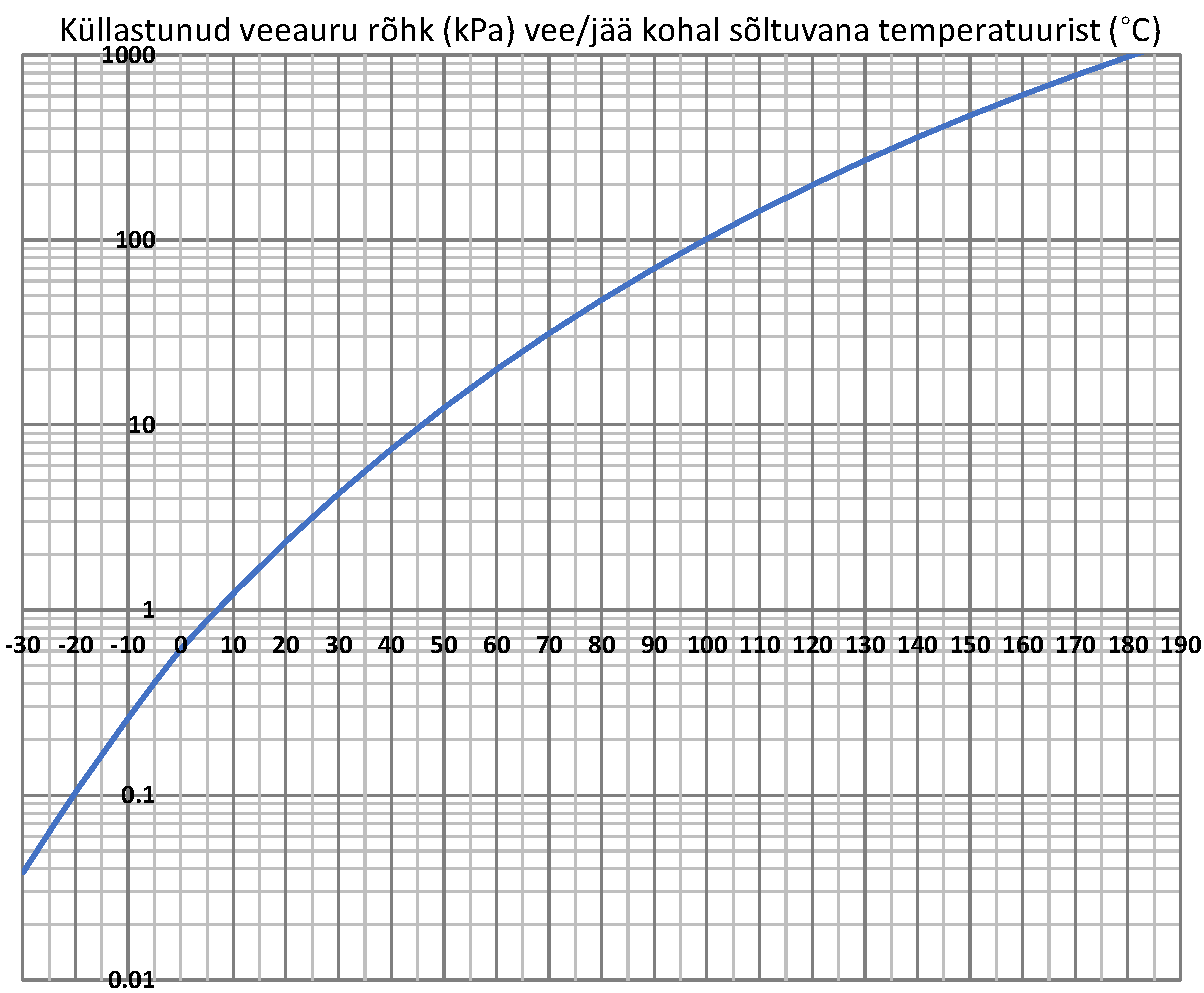
\includegraphics[width=0.95\textwidth]{veeaur.pdf}
  \vspace{-1em}
\end{figure}

\yl{SOOLVESI}
Silindriline anum on täidetud kõrguseni $H=\SI{20}{cm}$ soolveega, mille tihedus on $\rho_s=\SI{1.25}{g/cm^3}$. Silindrisse visatakse magedast veest tehtud jääkuubikuid sellisel hulgal, et vedeliku kõrgus anumas tõuseb $h=\SI{10}{cm}$ võrra. Kui palju (ja millises suunas) muutub vedeliku tase silindris, kui kogu jää on ära sulanud ja mage vesi soolveega ära segunenud? Mageda vee tihedus  $\rho_v=\SI{1.00}{g/cm^3}$ ning jää tihedus  $\rho_j=\SI{0.90}{g/cm^3}$. Lugeda, et soolvee tiheduse erinevus mageda vee omast on võrdeline soola protsentuaalse sisaldusega soolvees. \\
\emph{Märkus:} kõiki arvandmeid ei pruugi vaja minna.
\punktid{8} \autor{Jaan Kalda}

\newpage
\yl{KAUGUSVISE} Mis nurga all tuleb ühtlase kaldega pinnal (kaldenurk $\alpha$) visata, et pall lendaks fikseeritud algkiiruse juures võimalikult kaugele?
\punktid{10} \autor{Jaan Kalda}

\yl{HANTEL} Kaks pisikest kera, kumbki massiga $m$, on ühendatud üksteise külge kerge jäiga varda abil, mille pikkus on $l$; nimetagem seda süsteemi edaspidi hantliks. Üks kera kannab laengut $q$, kuid teine on ilma laenguta. Alghetkel on hantel horisontaalne ning liikumatu ja asub vertikaalses elektriväljas tugevusega $E$; raskusväli puudub. Milline on hantli telje pöörlemise maksimaalne nurkkiirus $\omega$ edasise liikumise käigus?
\punktid{10} \autor{Jaan Kalda}

\yl{OBERTHI EFEKT} Kosmoselaev tiirleb algselt ümber planeedi ringorbiidil raadiusega $r_0=\SI{70000}{km}$. Kosmoselaeva joonkiirus on $v_0=\SI{3}{\km\per\s}$. Lühikese aja jooksul antakse kosmoselaevale liikumissuunaga vastupidine kiiruse muut $\Delta v=\SI{1}{\km\per\s}$, mille tulemusena on kosmoselaev nüüd elliptilisel orbiidil. Kui kosmoselaev on oma orbiidil planeedile lähimas punktis, siis antakse sellele lühikese aja jooksul liikumissuunaline kiiruse muut $\Delta v=\SI{1}{\km\per\s}$.\\
\osa Mis on kosmoselaeva ja planeedi keskme vaheline kaugus $r_1$ teise manöövri hetkel?\\
\osa Mis on kosmoselaeva joonkiirus $v_2$, kui see on pärast teist manöövrit planeedist uuesti kaugusel $r_0$?\\
\emph{Vihje:} Gravitatsioonivälja potentsiaalne energia avaldub kujul $E_\text{pot} = -\frac{GMm}{r}$, kus $G$ on gravitatsioonikonstant, $M$ on planeedi mass, $m$ on kosmoselaeva mass ja $r$ kosmoselaeva kaugus planeedi keskmest. Samuti kehtib orbiitide jaoks impulsimomendi $L=mv_\perp r$ jäävuse seadus, kus $v_\perp$ on kiiruse tangentsiaalne (raadiusvektoriga risti olev) komponent.
\punktid{10} \autor{Eero Vaher}

\yl{PIDURDAV JALGRATAS}
Jalgrattur paneb libedal pinnasel sõites tähele, et kui ta esipiduri põhja vajutab, siis esiratas lõpetab pöörlemise ja jalgratas libiseb edasi kiirendusega $-a_1$. Tagaratas püsib libisemise käigus samuti maapinnal (ja pöörleb edasi). Kui ta esipiduri asemel tagapiduri põhja vajutab, siis tagaratas lõpetab pöörlemise ja jalgratas libiseb edasi kiirendusega $-a_2$.

Jalgrattast ja jalgratturist koosneva süsteemi massikeskme kõrgus on $h$ ja selle horisontaalkaugus kummagi ratta keskpunktist on $\ell$. Nii esi- kui tagaratta ja maapinna vaheline hõõrdetegur on $\mu$. Võite eeldada, et jalgratta kummagi ratta mass on võrreldes süsteemi massiga tühine.\\
\osa Leidke, millist võrratust peab rahuldama hõõrdetegur $\mu$, et esipiduri põhja vajutamise ajal tagaratas maast üles ei tõuseks.\\
\osa Leidke $\frac{a_1}{a_2}$.
\punktid{12} \autor{Kaarel Hänni}

\yl{KOLMNURK}
Traadist on tehtud võrdkülgne kolmnurk, mille sisse on pandud lõputult palju samast traadist tehtud võrdkülgseid kolmnurki (vt joonist). Traadi takistus pikkusühiku kohta on selline, et kolmnurga $ABC$ ühe külje takistus on $R$. Leidke kolmnurga $ABC$ tippude $A$ ja $B$ vaheline takistus.
\punktid{12} \autor{Kaarel Kivisalu}

\begin{figure}[h]
  \centering
  \begin{tikzpicture}[scale=3]
    \draw (0,0) node[left] {$A$} -- (2,0) node[right] {$B$}-- (1, 1.732) node[above] {$C$} -- (0,0);
    \foreach \x in {0,...,7}
    {
      \draw[line cap = round] (1, 1.734-1.732/2^\x) -- (1.003-0.5/2^\x,1.732-0.866/2^\x) -- (0.997+0.5/2^\x,1.732-0.866/2^\x) -- (1, 1.734-1.732/2^\x);
    }
  \end{tikzpicture}
\end{figure}

\end{document}

%%% Local Variables:
%%% mode: latex
%%% TeX-engine: default
%%% TeX-master: t
%%% End:
